%
%picaufbau
\subsection{Versuchsaufbau}
	\begin{figure}[h]
		\begin{center}
		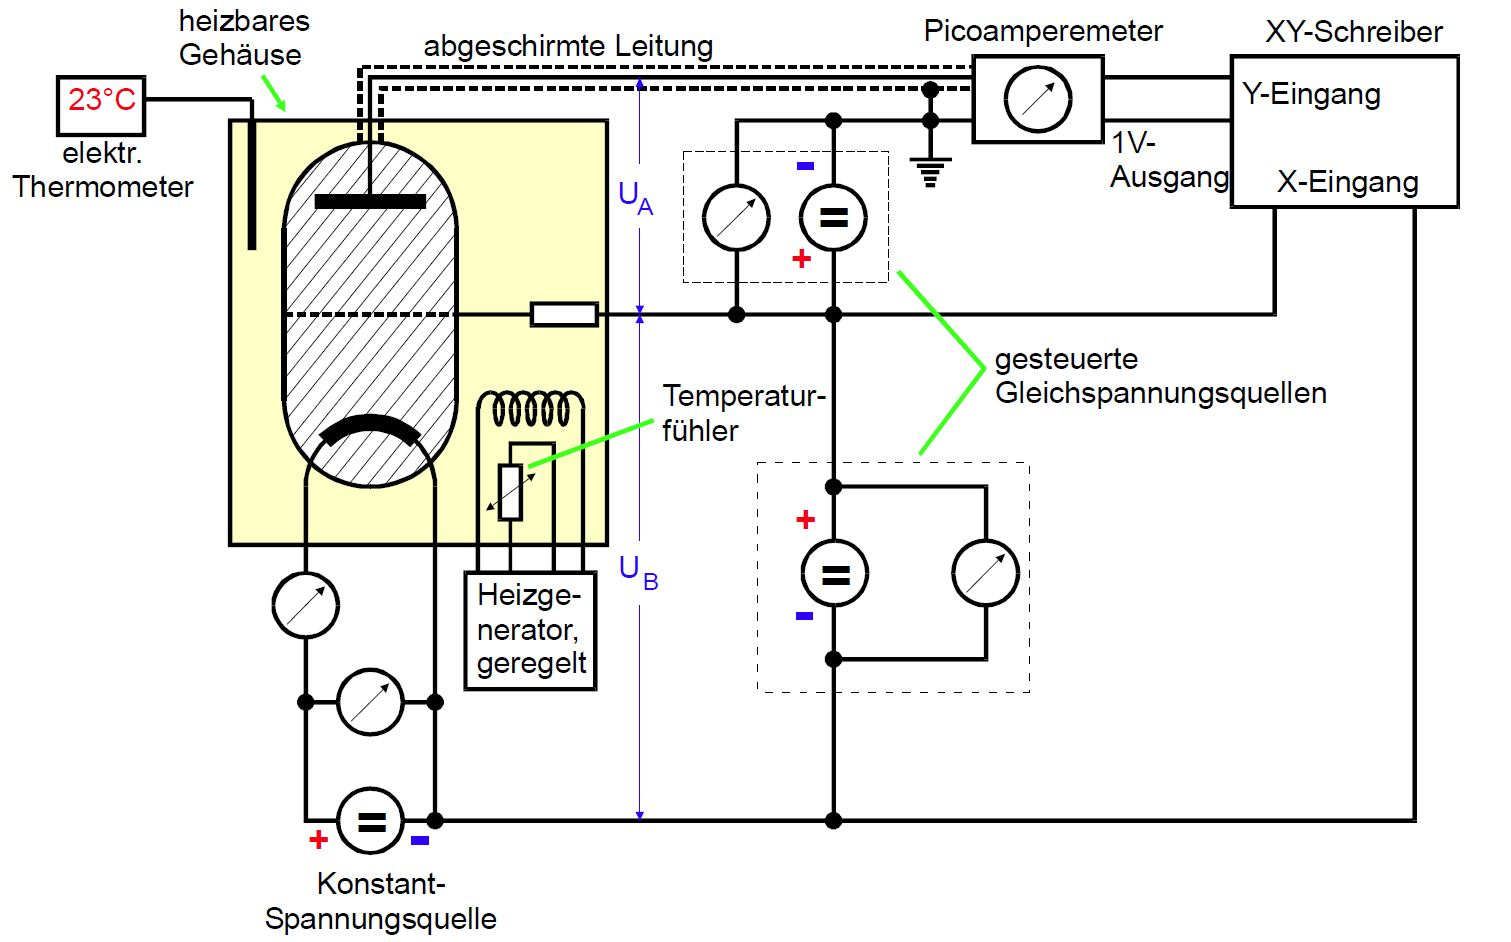
\includegraphics[scale=0.3]{picaufbau.jpg}
		\caption{Versuchsschaltung [1]}
		\label{picaufbau}
		\end{center}	
	\end{figure}
Der Versuch wird wie in Abbildung \ref{picaufbau} aufgebaut, sodass
die Aufnahmen für die folgenden Versuchsteile aufgezeichnet werden können.
An die oben beschriebenen Röhre (\ref{theorie}) werden Beschleunigungsspannung
und Abbremsspannung mit zwei steuerbaren Gleichspannungsquellen angelegt und der
Auffängerstrom wird über ein Picoampermeter  mit dem Y-Eingang des XY-Schreibers
verbunden. An den X-Eingang wird je nach Versuch entweder die Beschleunigungsspannung
oder die Abbremsspannung angelegt. Desweiteren befindet sich ein Thermometer in dem 
heizbaren Gehäuse der Röhre, welches über einen regelbaren Heizgenerator beheizt wird.
\subsection{Betimmung der Energieverteilung der beschleunigten Elektronen}
Nachdem der X-Y-Schreiber auf das aufzuzeichnende Intervall kalibriert ist, wird
bei konstantem Beschleunigungsstrom und
bei Zimmertemperatur, beziehungsweise bei erhöhter Temperatur
jeweils der Auffängerstrom in Abhängigkeit der Abbremsspannung aufgezeichnet.
\subsection{Bestimmung der Franck-Hertz-Kurve}
Nachdem der X-Y-Schreiber auf das aufzuzeichnende Intervall kalibriert ist, wird
bei passender Temperatur und konstanter Abbremsspannung der Auffängerstrom in 
Abhängigkeit der Beschleunigungsspannung 
aufgezeichnet, sodass deutlich genug Maxima zu erkennen sind.
\subsection{Bestimmung der Ionisierungsspannung von Hg}
Nachdem der X-Y-Schreiber auf das aufzuzeichnende Intervall kalibriert ist, wird
bei hoher Abbremsspannung und erhöhter Temperatur der Auffängerstrom in Abhängigkeit 
der Beschleunigungsspannung aufgezeichnet.